\section{Problem no.1}

The task is to design a corporate beam forming network that provides the correct power distribution to each radiating element. The microstrip design is carried on considering FR4 as substrate, whose technological specifications follow in table \ref{tab:p1_FR4}.

 \begin{table} [b]
 	\label{tab:p1_FR4}
 	\caption{FR4 technological specifications.}
 	\centering	
 	\begin{tabular}{lrrr} 
 		\toprule 
 		Quantity & Symbol & value & \\
 		\midrule
		Dielectric permittivity &$\epsilon_{r}$		&4.3		& 		\\
 		Substrate height&	h				& 1.5		&  mm	\\ 
 		Metal thickness&t	& 0.1	& mm\\
 		Minimum strip width &W\textsubscript{min}&0.15 & mm \\
 		Minimum spacing between lines &$\Delta$s\textsubscript{min}&0.175 & mm \\
 		\bottomrule 
 	\end{tabular}	
 \end{table}

The antenna's radiating part requires four radiators with cosine-over-pedestal tapering, hence the BFN is symmetric with respect to the feeding line. %What follows is the theoretical design for the network, whose final optimized solution is presented in the following section. 

\begin{figure}[t] 
	\centering
	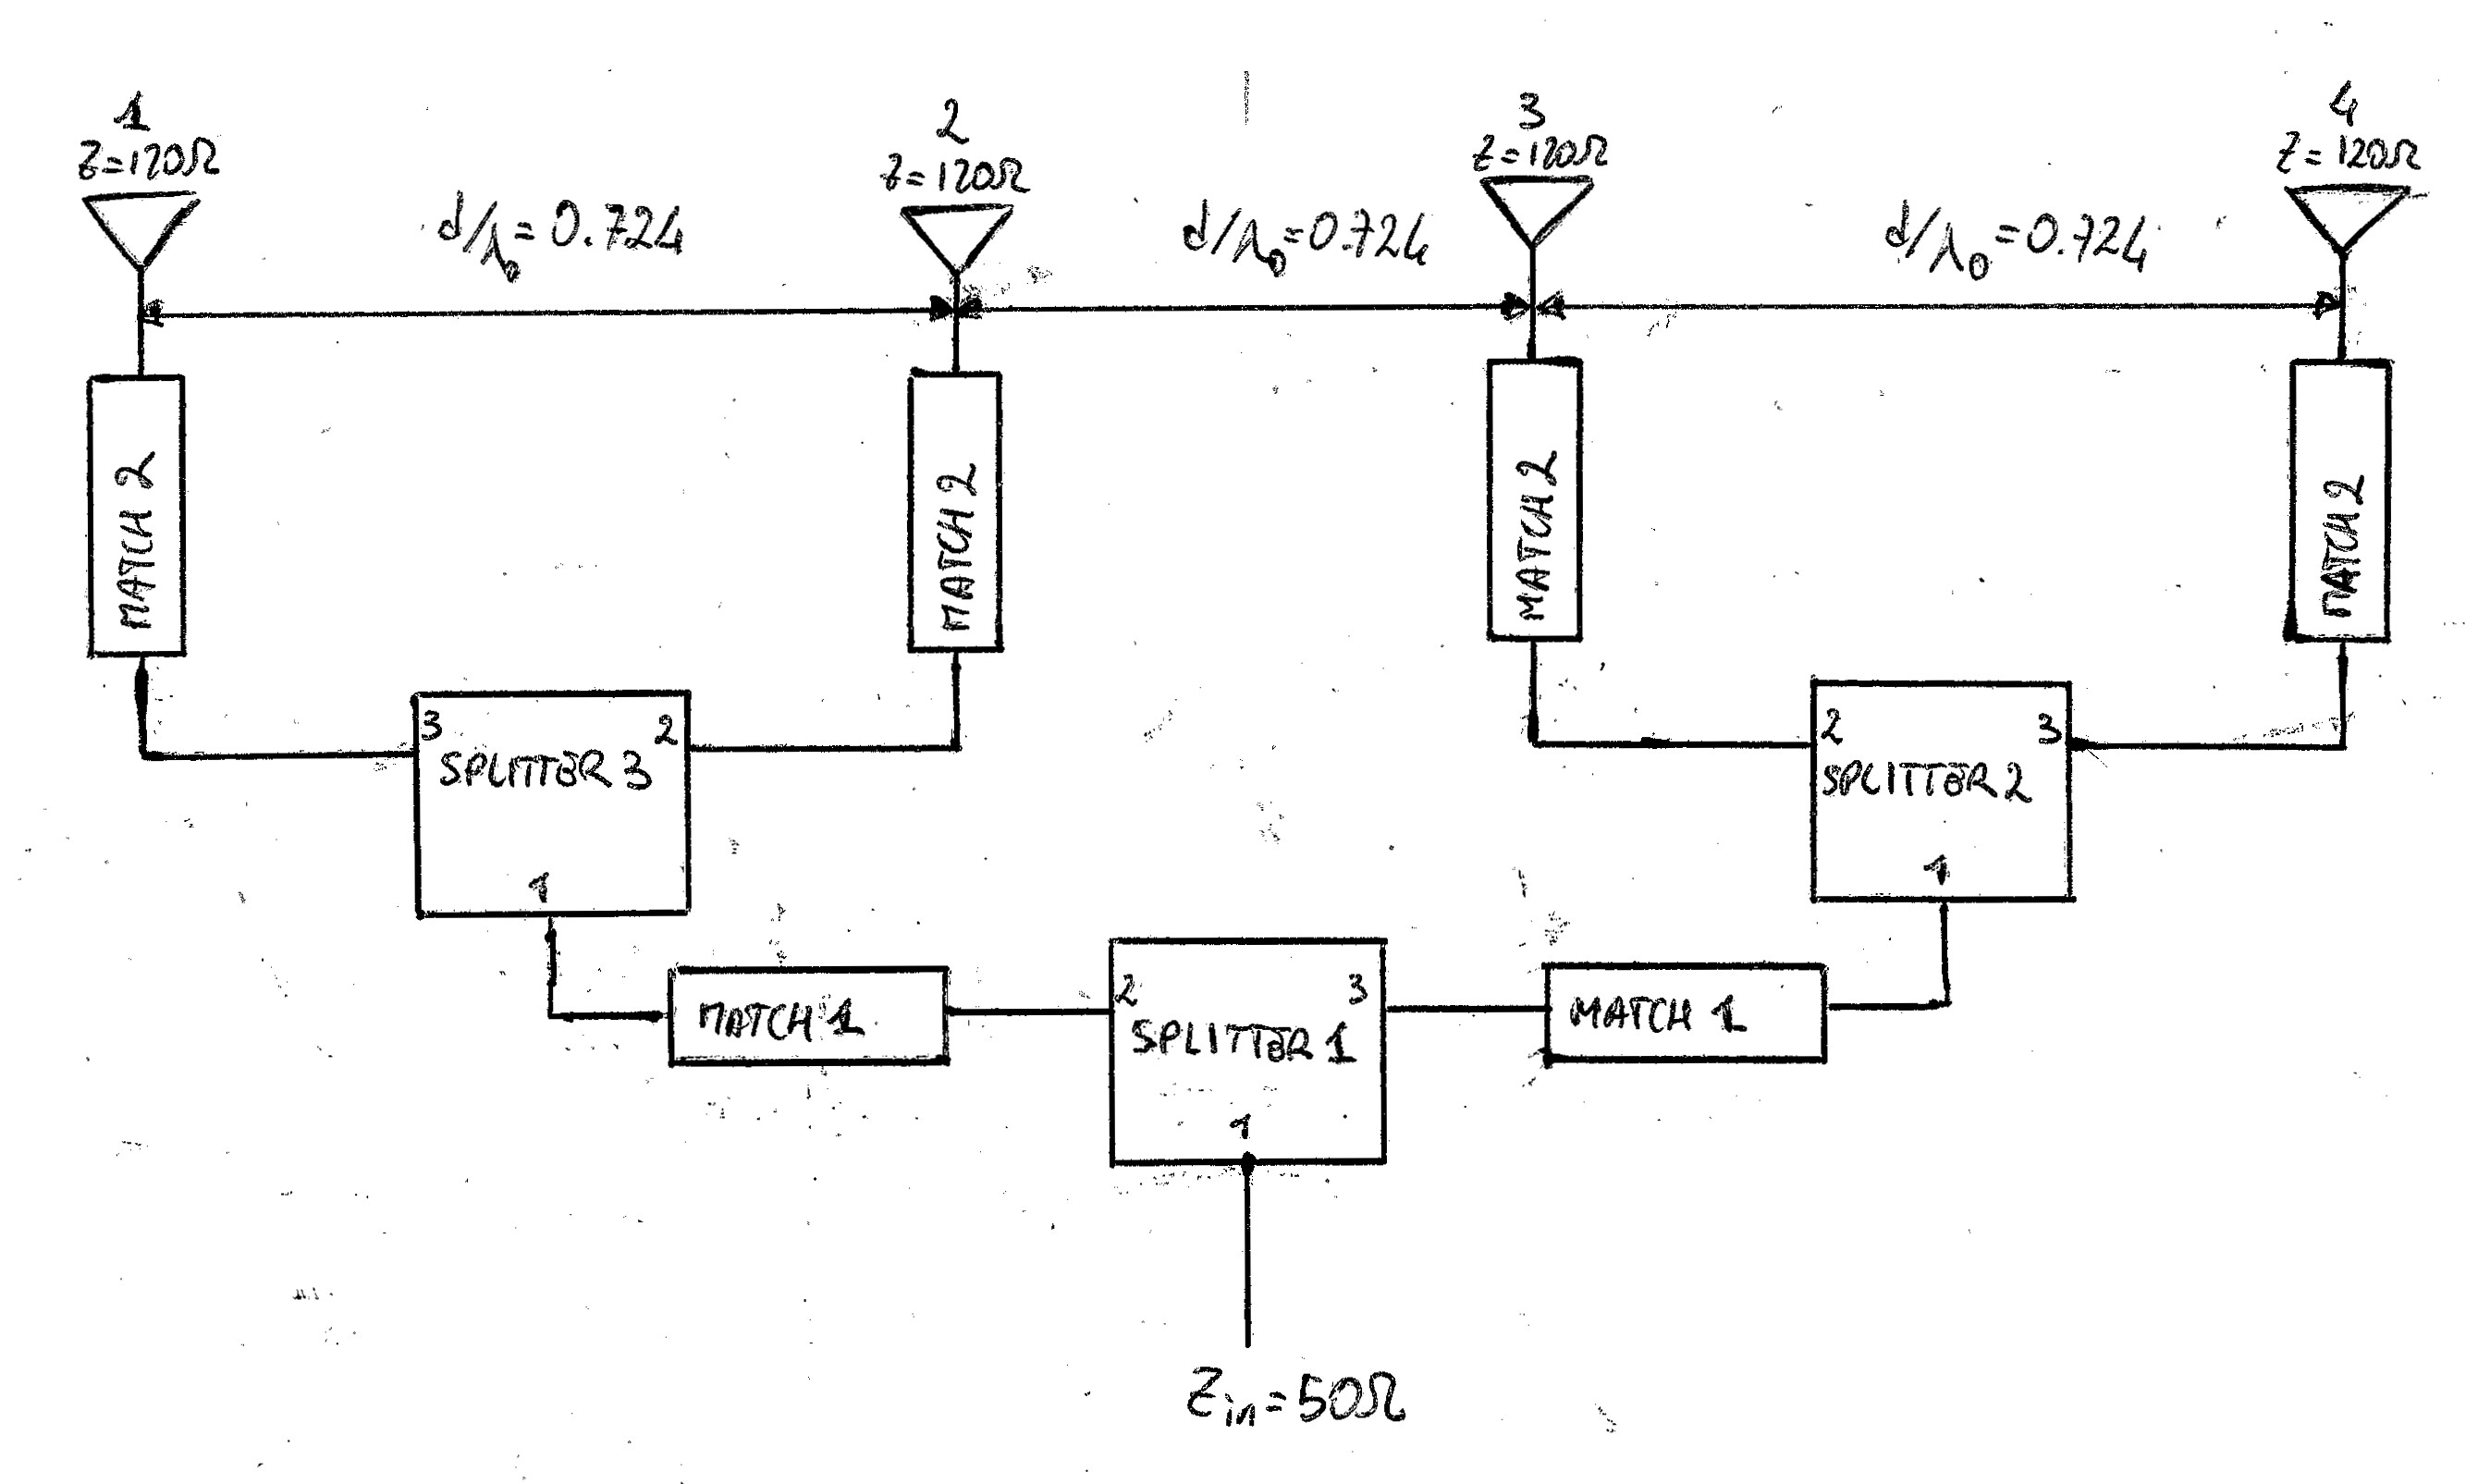
\includegraphics[scale=0.5]{p1_bfn_block}
	\caption{Beam forming network block diagram.}
	\label{fig:p1_bfn_block}
\end{figure}

One possible implementation is proposed in figure \ref{fig:p1_bfn_block}, where the building blocks can be identified as follows: 
\begin{description}
	\item [Splitter1] this section matches the input line to Z\textsubscript{in}=50$\Omega$ at the input port. Moreover, it evenly splits the power into the two following branches, therefore the power splitter is a 3dB splitter. 
	\item [Splitter2] this section matches the radiating elements with section1 outputs, moreover it convey power into the radiators giving the correct power ratio between elements.
	\item [Splitter3] this is symmetric to section2 with respect to the feeding line longitudinal axis. 
	\item [Match1] these lines acts as matching connection from power splitter1 to power splitters2 and 3, moreover they are used to adjust the distance between elements.
	\item [Match2] matching connections between radiators and power splitters2,33;
\end{description}
Overall the BFN must be designed in order to be compliant with the requirement on:
\begin{itemize}
	\item grating lobes, then the element spacing d (d/$\lambda_0=0.724$);
	\item amplitude tapering between edge and centre elements;
	\item main beam direction: since the array is broadside then the phase shift among elements must be null.
\end{itemize}
Each block's design and simulation are reported in the following paragraphs.

\subsection{Splitter 1 design}

Figure \ref{fig:p1_sec1_block} shows the block diagram of splitter1. 
\begin{figure}[H] 
	\centering
	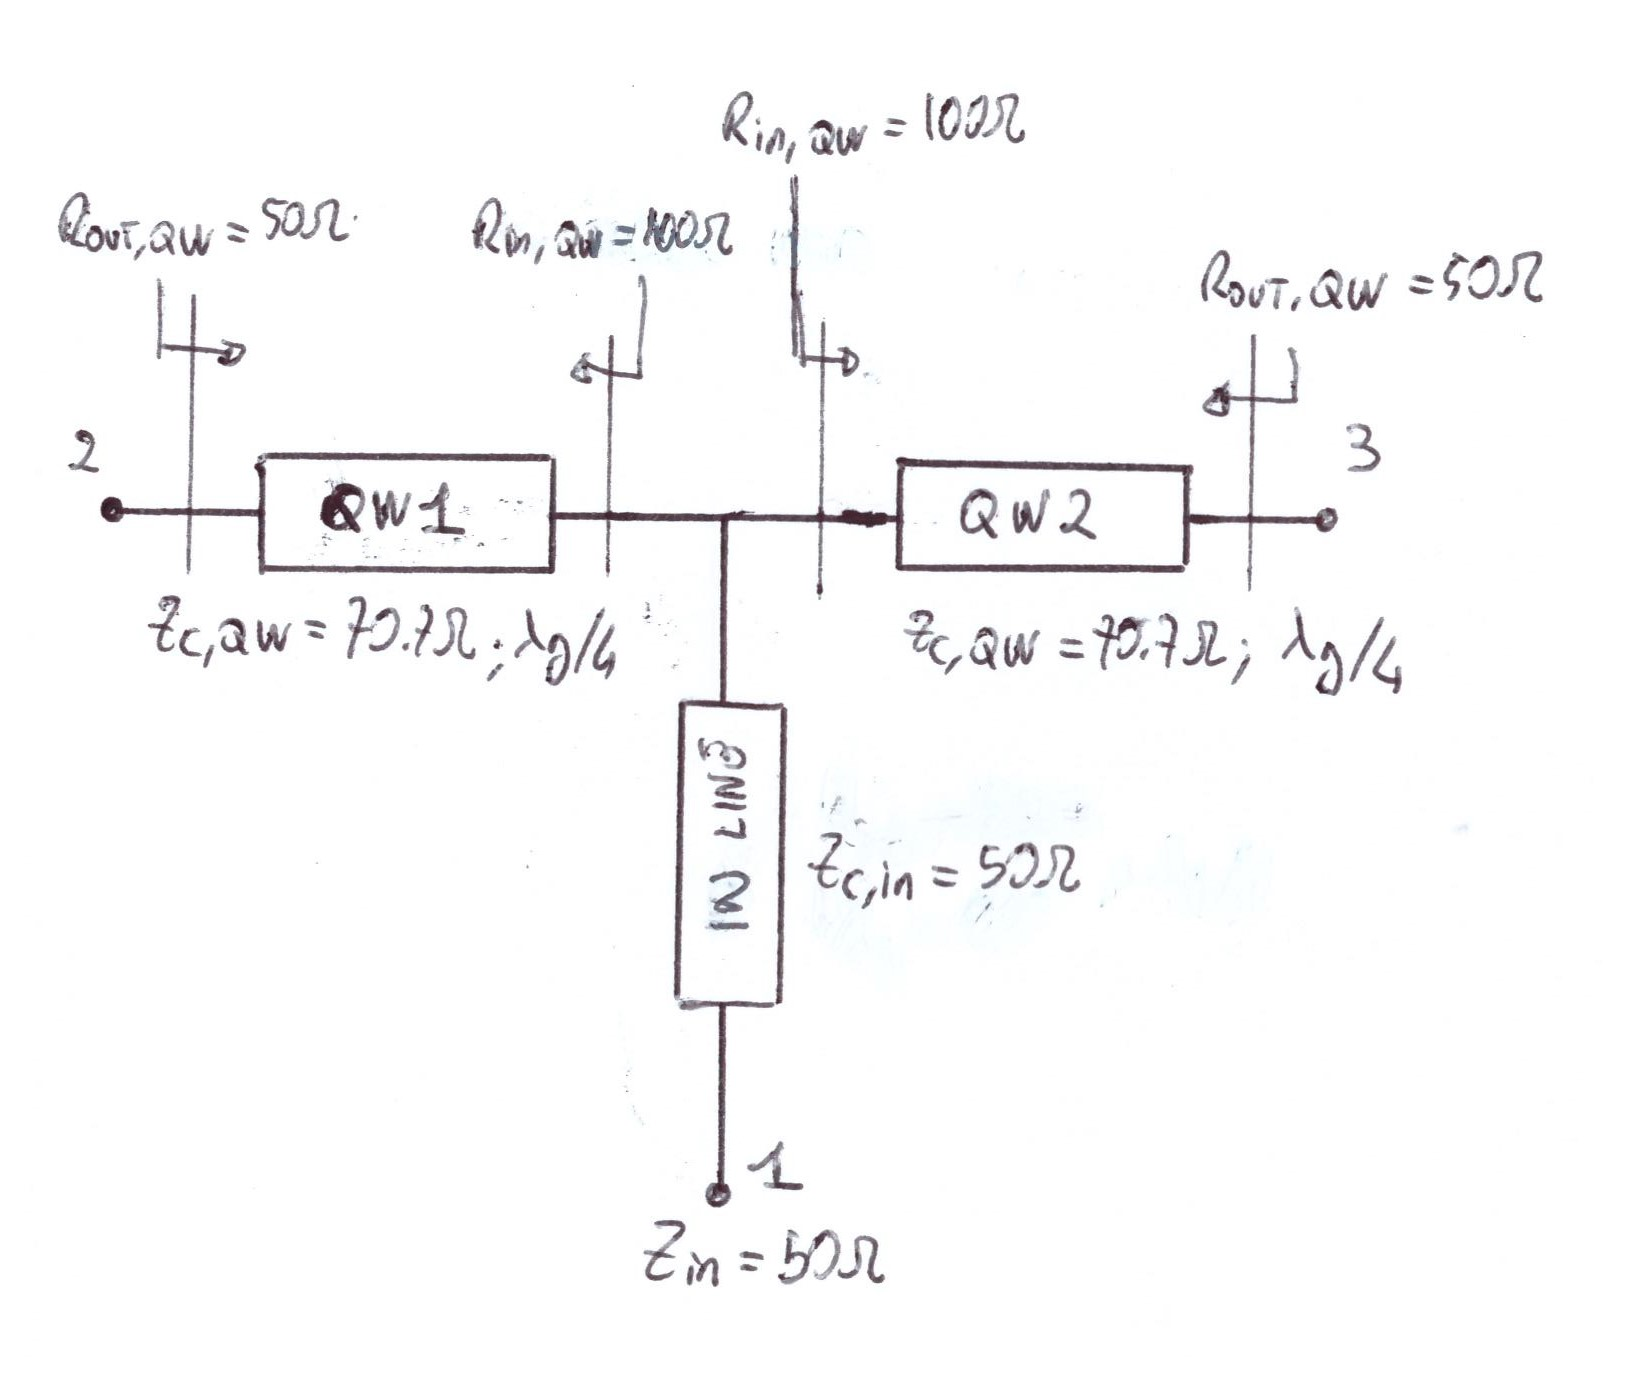
\includegraphics[scale=0.5]{p1_sec1_bl}
	\caption{Splitter1 TXL implementation. }
	\label{fig:p1_sec1_block}
\end{figure}
The input line is matched to the input port by means of a 50$\Omega$ line whose length has been chosen equal to $\lambda_{g}/4$. To evenly split the power into port 2 and 3 we use a T-junction made up of two quarter-wavelength transformers. This components show real input and output impedance and the following relation for their characteristic impedance holds:
\begin{equation}
	\label{eq:p1_ZcQW}
	Z_{c,QW} =R_{c,QW}=\frac{1}{G_{c,QW}}= \sqrt{R_{in,QW}\cdot R_{out,QW}} 
\end{equation}
The two quarter-wavelength transformers are seen as two parallel admittances from the input port, then to have the 50$\Omega$ matching we have:
\begin{equation}
	G_{c,QW1}+G_{c,QW2}=\frac{1}{Z_{in}}=\frac{1}{50\Omega} \; \Rightarrow \; Z_{c,QW1}=Z_{c,QW2}=Z_{c,QW}=100\Omega \notag
\end{equation}
 Willing to reduce impedance discontinuities within the network, the section's output impedance is set to 50$\Omega$ too, hence:
\begin{equation}
	Z_{c,QW}= \sqrt{R_{in,QW}\cdot R_{out,QW}}=\sqrt{100\Omega\cdot 50\Omega}=70.7\Omega \notag
\end{equation}
\begin{figure}[H] 
	\centering
	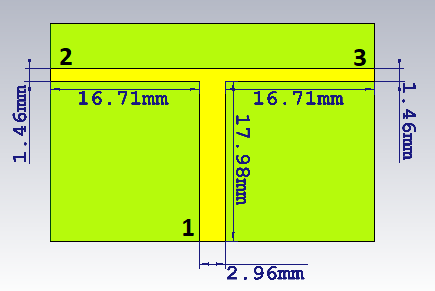
\includegraphics[scale=0.5]{p1_sec1_ustrip}
	\caption{Splitter1 microstrip implementation. }
	\label{fig:p1_sec1_ustrip}
\end{figure}
Finally the design has been converted from ideal microstrip lines to physical lines by means of TX-LINE: Transmission Line Calculator (from NI AWR Design Environment) and eventually implemented in CST DS\texttrademark{} for the optimization process. 
Theoretical and optimized dimensions are reported in table \ref{tab:p1_sec1DimIN} and\ref{tab:p1_sec1DimIN}. The resulting scattering parameters are shown in figure \ref{fig:p1_sec1Scatt}: both power splitting and phase behaves as expected. Figure \ref{fig:p1_sec1_ustrip} depicts the microstrip implementation of this section.
\begin{table} [H]
	\label{tab:p1_sec1DimIN}
	\caption{Splitter1: Input line dimensions}
	\centering	
	\begin{tabular}{lccc} 
		\toprule
			& theoretical & optimized&\\
		\midrule 
		W\textsubscript{in} 	&	3.020		&	2.964	 & mm 		\\
		L\textsubscript{in}		&	16.797		& 	17.976		& mm	\\ 
		Z\textsubscript{c,in}	& 	50 & 50.6	&$\Omega$ \\
		\bottomrule
	\end{tabular}	
\end{table}
\begin{table} [H]
	\label{tab:p1_sec1DimQW}
	\caption{Splitter1: quarter-wavelength transformer dimensions}
	\centering	
	\begin{tabular}{lccc} 
		\toprule
		& theoretical & optimized&\\
		\midrule 
		W\textsubscript{QW} 	&	1.599		&	1.458	& mm		\\
		L\textsubscript{QW}	&	17.248		& 	16.706		& mm	\\ 
		Z\textsubscript{c,QW}& 	70.7 &73.9	&$\Omega$ \\
		\bottomrule
	\end{tabular}	
\end{table}
\begin{figure}[p] 
	\centering
	\subfloat[][\emph{Modulus}]{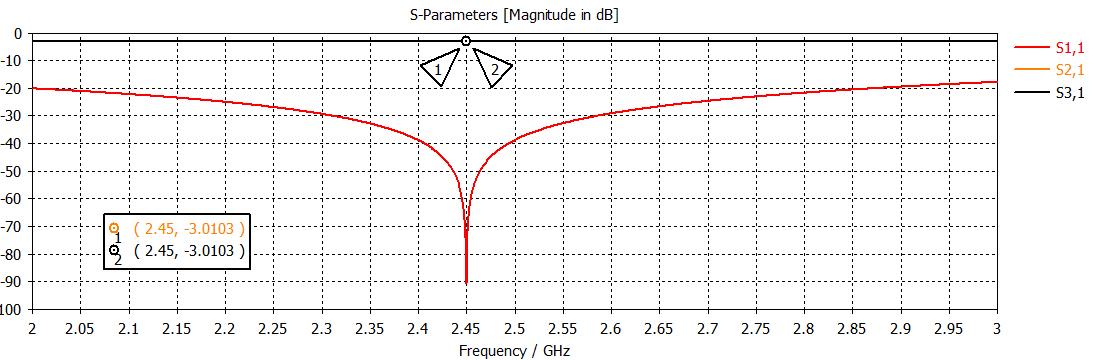
\includegraphics[scale=.6,angle=90]{p1_sec1_Smod}}\quad
	\subfloat[][\emph{Phase}]{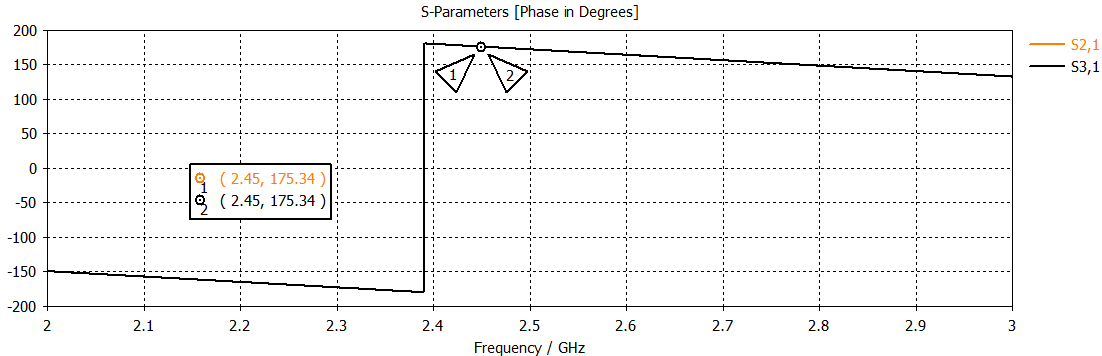
\includegraphics[scale=.6,angle=90]{p1_sec1_Sph}}\\
	\caption{Section 1 most important scattering parameters. As it appears both input matching and even power splitting are accomplished, the phase shift is null (reference impedance 50$\Omega$).}
	\label{fig:p1_sec1Scatt}
\end{figure}
\newpage

\subsection{Splitters2,3 and match2 design}

Figure \ref{fig:p1_sec2_block} shows the block diagram of splitter2 and match1 (splitter3  and match1 are specular).
\begin{figure}[H] 
	\centering
	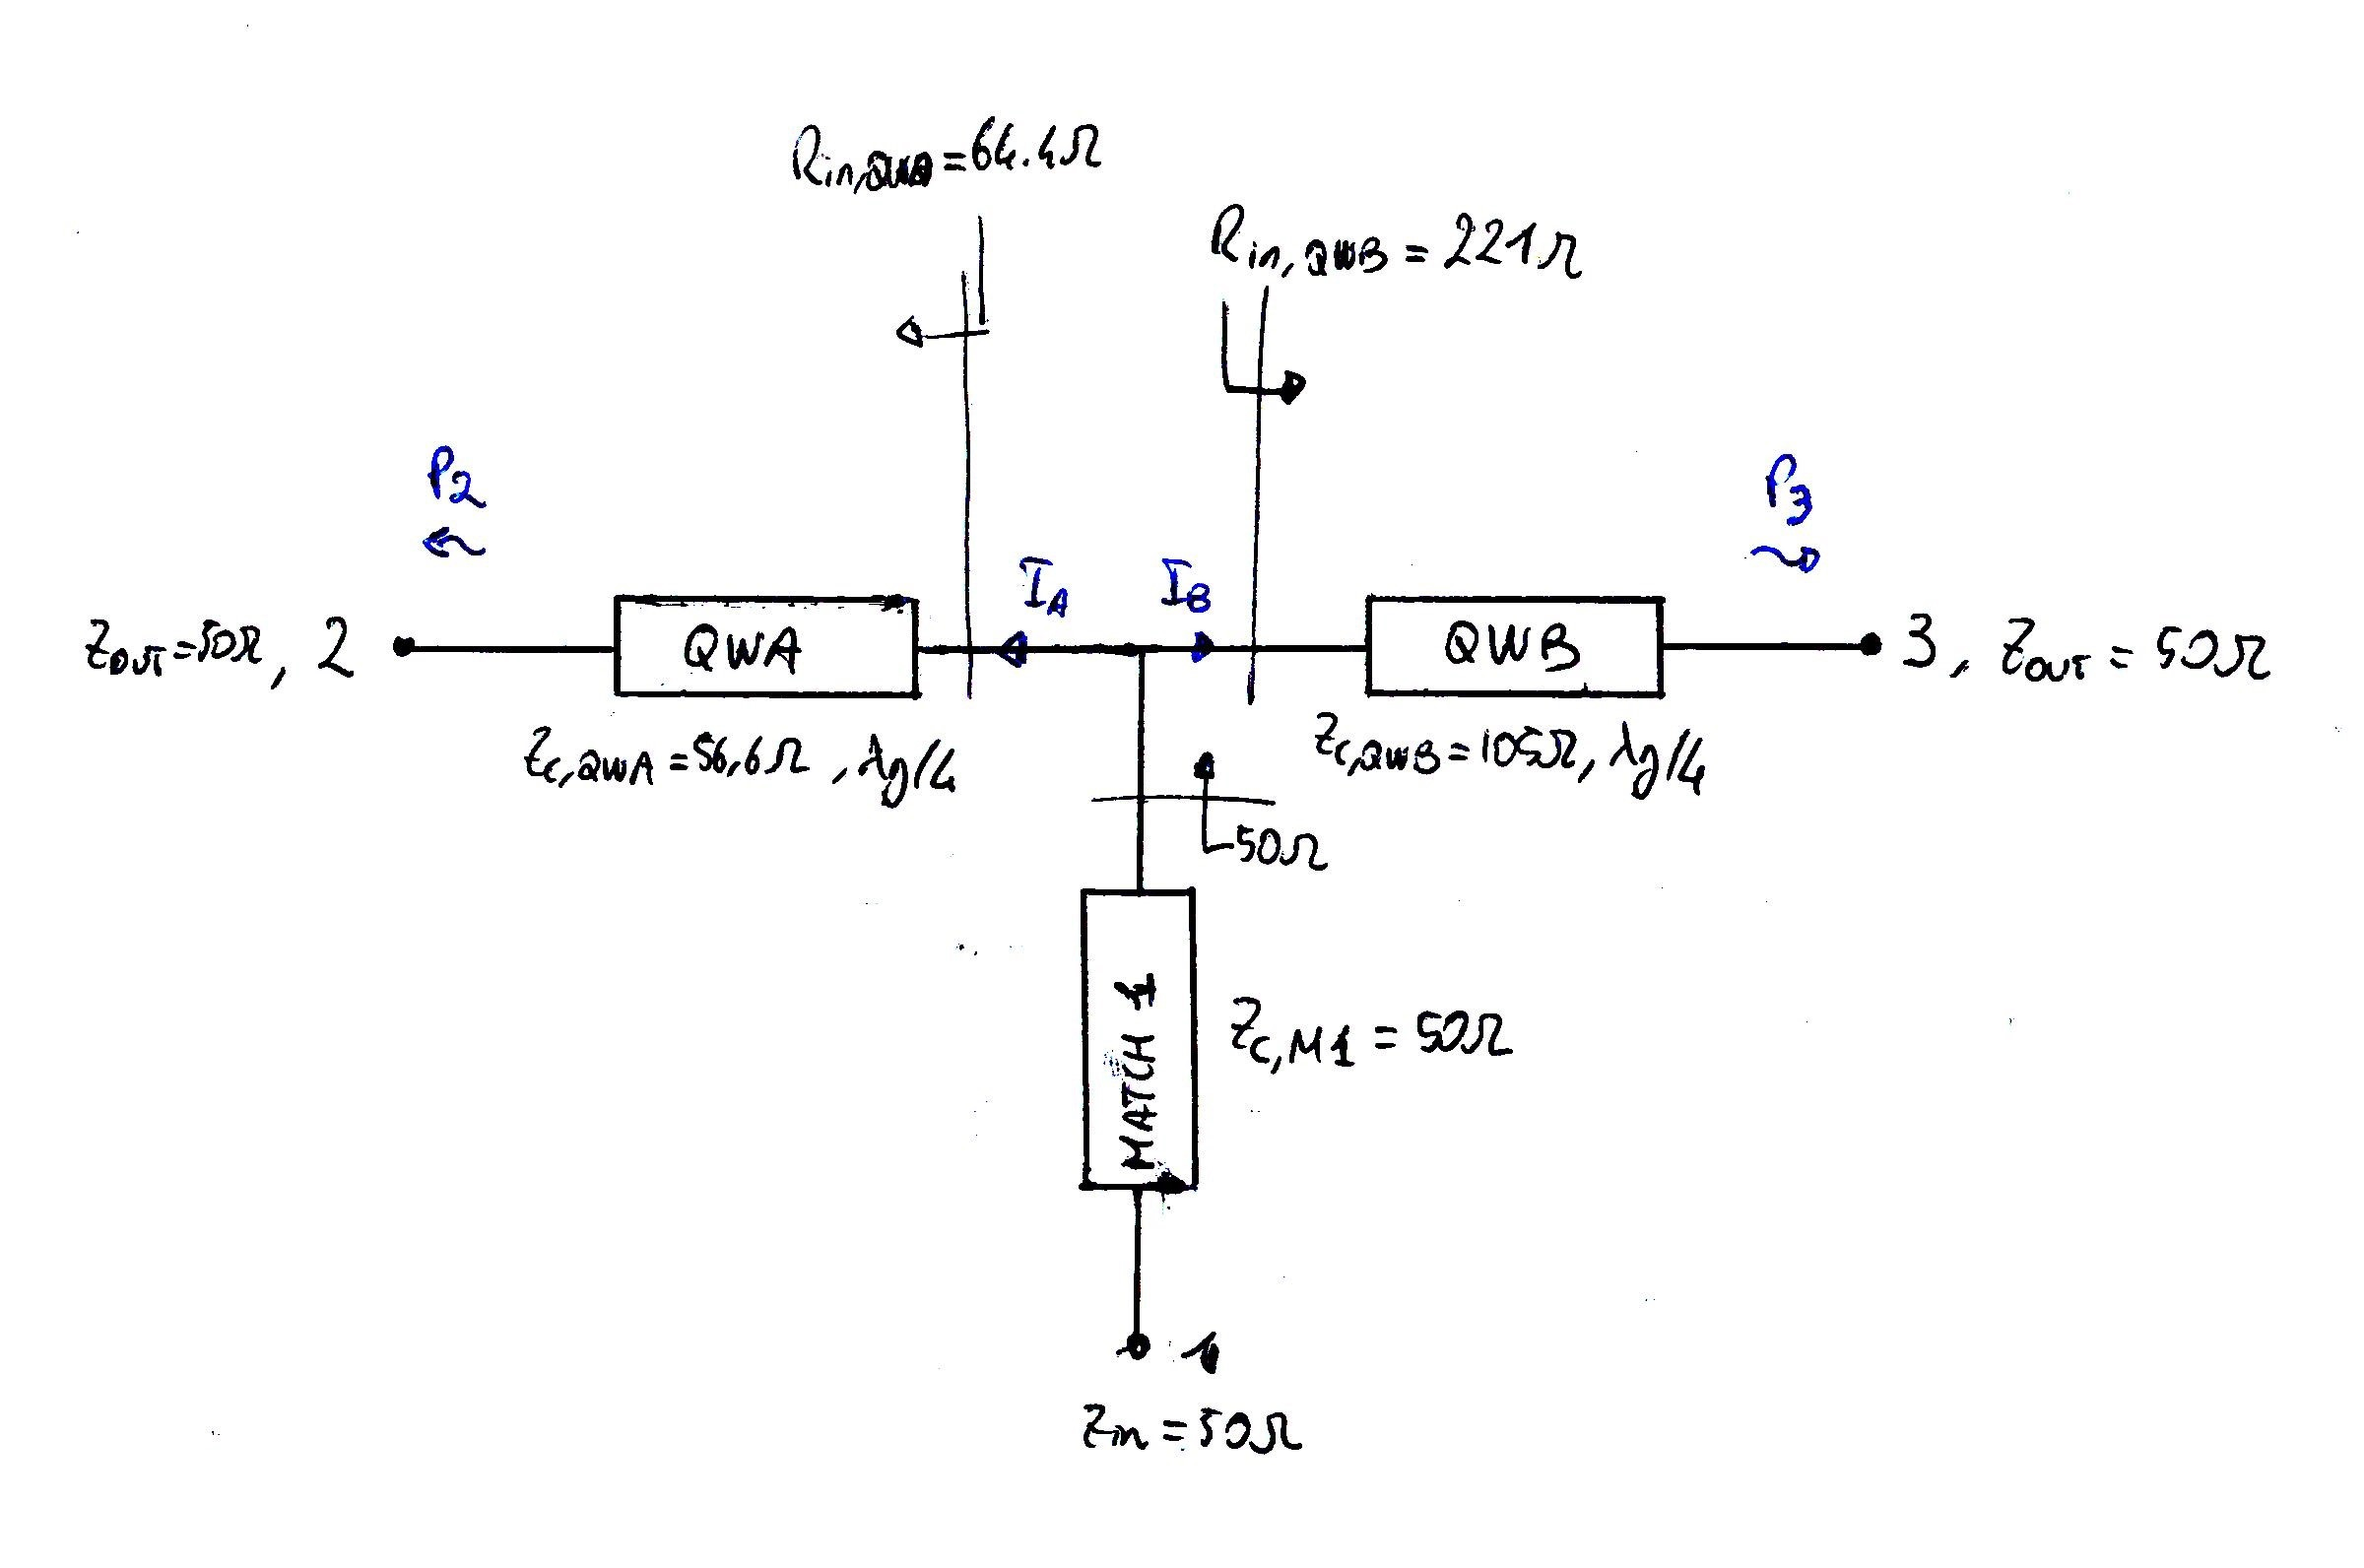
\includegraphics[scale=0.5]{p1_sec2_block}
	\caption{Splitter2 and match1 TXL implementation. }
	\label{fig:p1_sec2_block}
\end{figure}
Match1 lines are designed as $\lambda_{g}/2$, 50$\Omega$ characteristic impedance microstrip lines. Acting as transparent transmission lines, they allow splitter2 and 3 to have Z\textsubscript{in}=50$\Omega$ at their input ports. Again a Z\textsubscript{out}=50$\Omega$ is chosen to avoid abrupt impedance variations. Imposing Z\textsubscript{in}=50$\Omega$ we also avoid the appearance of lines narrower than W\textsubscript{min} within the power splitter2 (and splitter3).

The splitter is composed by two quarter-wavelength transformers that provide the correct current tapering for the radiators. To design that we will consider the power entering and exiting the component.
Having chosen as tapering t=0.54, then:
\begin{equation}
	\frac{S_{31}}{S_{21}}=0.54 \; \Rightarrow \; \frac{P_3}{P_2}=\Bigg(\frac{S_{31}}{S_{21}}\Bigg)^2=0.292 \Rightarrow \frac{P_3}{P_2}=-5.34dB \notag
\end{equation} 
where S\textsubscript{21} and S\textsubscript{31} are the scattering transmission coefficients at port 2 and 3. In particular P\textsubscript{2} is the power exiting the splitter and directed to the centre element, whereas P\textsubscript{3} is goes to the edge radiator (supposing lossless TXL):
\begin{equation}
	\begin{cases}
		P_2 = P_a = \frac{1}{2}R_{in,QWa}|I_A|^2 \notag \\	
		P_3 = P_b = \frac{1}{2}R_{in,QWb}|I_B|^2 \notag	
	\end{cases}	
\end{equation}
As before, the two impedance transformers are seen as two in-parallel conductances from port 1, then the following system holds: 
\begin{equation}
	\begin{cases} 
		\frac{1}{R_{in,QWa}}+\frac{1}{R_{in,QWb}}=\frac{1}{Z_{in}} \notag\\
		\frac{P_{3}}{P_{2}}=\frac{R_{in,QWa}}{R_{in,QWb}}=0.292 \notag
	\end{cases}
\end{equation}
that has solutions:
\begin{gather}
	R_{in,QWb} = 221\Omega \notag \\
	R_{in,QWa} = 64.6\Omega \notag
\end{gather}
From equation (\ref{eq:p1_ZcQW}):
\begin{gather}
	Z_{c,QWb}=\sqrt{R_{in,QWb}\cdot Z_{out}}=\sqrt{221\Omega \cdot 50\Omega}=105\Omega \notag \\
	Z_{c,QWa}=\sqrt{R_{in,QWa}\cdot Z_{out}}=\sqrt{64.4\Omega \cdot 50\Omega}=56.7\Omega \notag
\end{gather}
The circuit has been then converted into microstrip layout and simulated. Optimized dimensions for this section are reported in table \ref{tab:p2_sec2DimM1}, \ref{tab:p2_sec2DimQWa} and \ref{tab:p2_sec2DimQWb}.
Unfortunately, the splitter2's values found so far produced a wrong tapering (t=-4.2dB), therefore the lines width and length have been tuned till the desired tapering specification has been fulfilled. Since t>-5.3dB we need to increase the difference between R\textsubscript{in,QWa} and R\textsubscript{in,QWb}. 
With t=-5.2dB we have the best compromise between excitation amplitude distribution and phase shift, that is equal to 3.94$^\circ$.
Figure \ref{fig:p2_sec1Scatt} shows the input parameters, while figure \ref{fig:p1_sec2_ustrip} depicts the microstrip implementation.
\begin{figure}[t] 
	\centering
	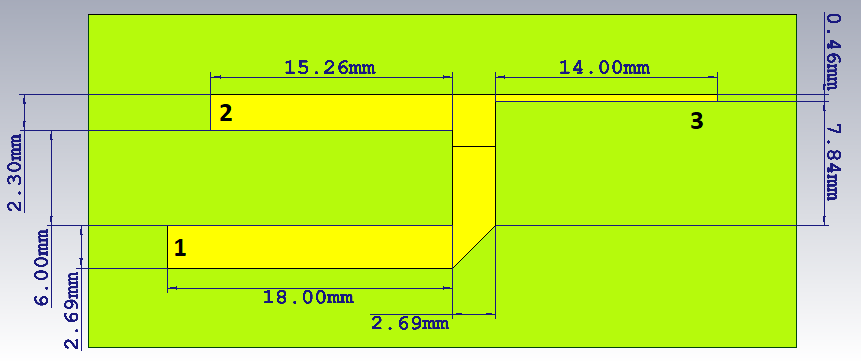
\includegraphics[scale=0.5]{p1_sec2_ustrip}
	\caption{Splitter1 microstrip implementation. }
	\label{fig:p1_sec2_ustrip}
\end{figure}
\begin{table} [H]
	\label{tab:21_sec2DimM1}
	\caption{Match1: microstrip dimensions.}
	\centering	
	\begin{tabular}{lcccc} 
		\toprule
		& theoretical & optimized (no tap)& optimized (tap)&\\
		\midrule 
		W\textsubscript{M1} 	&	3.021		&	2.964	&2.695& mm 		\\
		L\textsubscript{M1}		&	33.594		& 	33.594	&23.133& mm		\\ 
		Z\textsubscript{c,M1}	&	50			& 	50.6	&53.5& $\Omega$		\\
		\bottomrule
	\end{tabular}	
\end{table}
\begin{table} [H]
	\label{tab:p2_sec2DimQWa}
	\caption{Splitter2: quarter-wavelength a dimensions.}
	\centering	
	\begin{tabular}{lcccc} 
		\toprule
		& theoretical & optimized(tap) &optimized (tap)&\\
		\midrule 
		W\textsubscript{QWa} 	&	2.435		&	2.106	&2.295& mm		\\
		L\textsubscript{QWa}	&	16.959		& 	14.656	&15.262& mm		\\ 
		Z\textsubscript{c,QWa}	&	56.6		& 	61.4	&58.6& $\Omega$		\\
		\bottomrule
	\end{tabular}	
\end{table}
\begin{table} [H]
	\label{tab:p2sec2DimQWb}
	\caption{Splitter2: quarter-wavelength b dimensions.}
	\centering	
	\begin{tabular}{lcccc} 
		\toprule
		& theoretical & optimized(no tap) &optimized (tap)&\\
		\midrule 
		W\textsubscript{QWb} 	&	0.613		&	0.507	&0.457& mm		\\
		L\textsubscript{QWb}	&	17.709		& 	16.170	&14.005& mm		\\ 
		Z\textsubscript{c,QWb}	&	105			& 	112		&116& $\Omega$		\\
		\bottomrule
	\end{tabular}	
\end{table}
\newpage

\begin{figure}[H] 
	\centering
	\subfloat[][\emph{Modulus}]{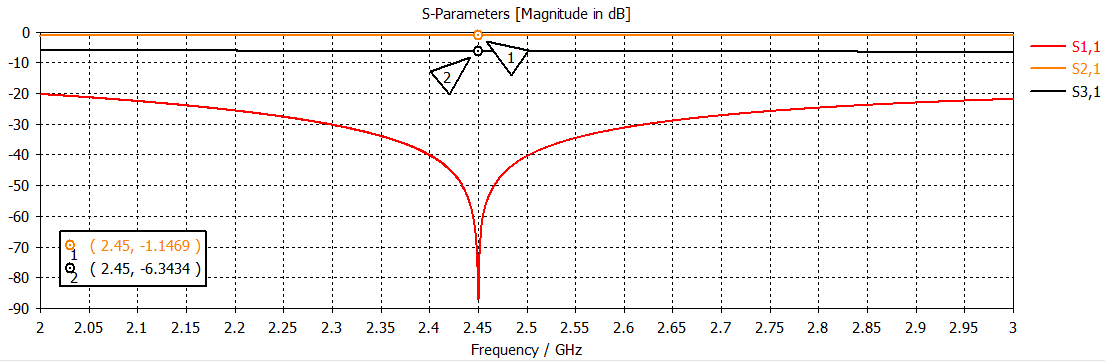
\includegraphics[scale=.6,angle=90]{p1_sec2_Smod}}\quad
	\subfloat[][\emph{Phase}]{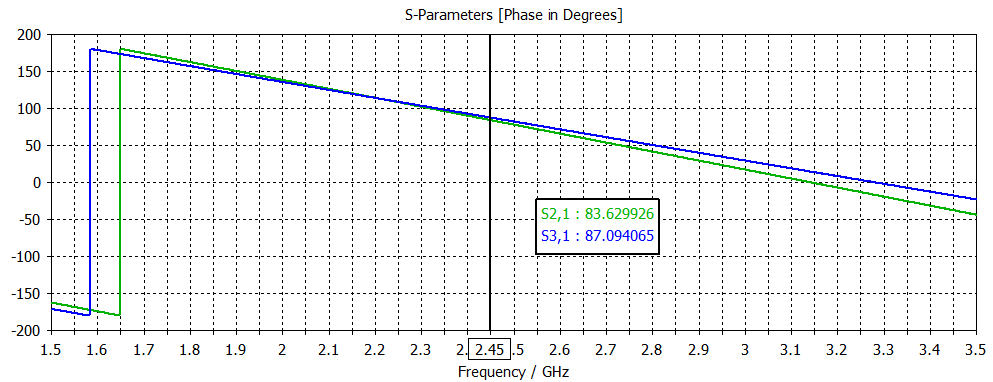
\includegraphics[scale=.6,angle=90]{p1_sec2_Sph}}\\
	\caption{Section 1 most important scattering parameters. As it appears both input matching and even power splitting are accomplished. The tapering value is t=-5.2dB, the phase shift amount to 3.94$^\circ$ (reference impedance 50$\Omega$).}.
	\label{fig:p2_sec1Scatt}
\end{figure}

\subsection{Match2 design}

As final design step another quarter-wavelength transformer is introduced. This element matches splitter2 and splitter3, R\textsubscript{out}=50$\Omega$, output impedance with the radiators' input impedance, equal to Z\textsubscript{in,patch}=120$\Omega$. Using equation (\ref{eq:p1_ZcQW}) we have:
\begin{align}
	Z_{c,M2}&=\sqrt{R_{in,M2}\cdot R_{out,M2}} \notag\\
	&=\sqrt{Z_{out}\cdot Z_{in,patch}} \notag\\
	&=\sqrt{120\Omega \cdot 50\Omega}=77.5\Omega \notag
\end{align}
The conversion from ideal microstrip to layout can be found in table \ref{tab:21_DimM2}, whereas the return loss is shown in figure \ref{fig:p1_M2_Smod}

\begin{table} [H]
	\label{tab:21_DimM2}
	\caption{Match2: microstrip dimensions.}
	\centering	
	\begin{tabular}{lccc} 
		\toprule
		& theoretical 			& optimized &\\
		\midrule 
		W\textsubscript{M1} 	&	1.316		&	1.212	& mm 		\\
		L\textsubscript{M1}		&	17.365		& 	17.365	& mm		\\ 
		Z\textsubscript{c,M1}	&	77.5		& 	80.45	& $\Omega$		\\
		\bottomrule
	\end{tabular}	
\end{table}

\begin{figure}[t] 
	\centering
	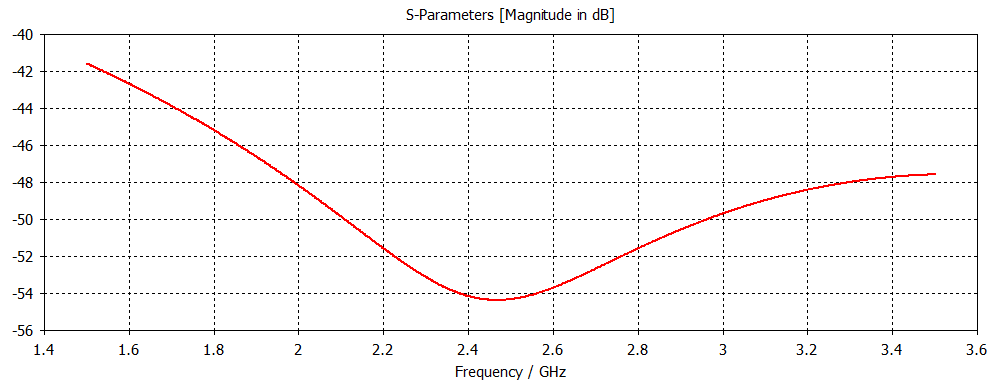
\includegraphics[scale=0.43]{p1_M2_Smod}
	\caption{Match2 return loss (reference impedance 50$\Omega$). }
	\label{fig:p1_M2_Smod}
\end{figure}